\chapter{Illumination, Materials, and Shading Pipeline}
\label{chap:lighting}

\section{The 16-Light Dynamic Optical Architecture}
The illumination pipeline in \textit{Matsuri Nights} models the complex nocturnal atmosphere of an illuminated festival street. Shaders operate in forward rendering with \textbf{16 active dynamic light sources}: 1 Directional Light (Sun/Moon), 14 Point Lights, and 1 Theatrical Spotlight. Table~\ref{tab:lights_catalog} provides the complete technical specification of every light source.

\begin{table}[htbp]
\centering
\scriptsize
\renewcommand{\arraystretch}{0.90}
\begin{tabularx}{\textwidth}{p{1.4cm} p{1.6cm} p{2.8cm} p{2.3cm} p{2.3cm} p{3.2cm}}
\toprule
\textbf{Light ID} & \textbf{Type} & \textbf{Physical Entity} & \textbf{Diffuse Color} & \textbf{Specular Color} & \textbf{Attenuation / Coupling} \\
\midrule
\textbf{DirLight} & Directional & Celestial Sun / Moon & Day: $(0.85, 0.82, 0.76)$ \newline Night: $(0.20, 0.25, 0.38)$ & Day: $(0.60, 0.60, 0.55)$ \newline Night: $(0.30, 0.35, 0.45)$ & Vector lerps $(0.4, -0.85, -0.5) \to (-0.35, -0.75, 0.4)$. Casts PCF shadows. \\
\addlinespace
\textbf{Point 0} & Point & Magic Orb & $(0.35, 0.85, 1.00)$ & $(0.50, 0.90, 1.00)$ & $k_l = 0.14, k_q = 0.07$. Tracks Magician hand bone. \\
\addlinespace
\textbf{Point 1} & Point & Takoyaki Stall Eaves & $(1.00, 0.60, 0.22)$ & $(1.00, 0.70, 0.30)$ & $k_l = 0.10, k_q = 0.045$. Pos: $(-5.2, 2.85, 6.0)$. \\
\addlinespace
\textbf{Point 2} & Point & Kakigori Stall Eaves & $(0.35, 0.90, 1.00)$ & $(0.50, 0.95, 1.00)$ & $k_l = 0.10, k_q = 0.045$. Pos: $(5.2, 2.85, 6.0)$. \\
\addlinespace
\textbf{Point 3} & Point & Street Lantern Span 1 & $(1.00, 0.55, 0.20)$ & $(1.00, 0.65, 0.25)$ & $k_l = 0.09, k_q = 0.032$. Tracks swinging lantern body. \\
\addlinespace
\textbf{Point 4} & Point & Street Lantern Span 3 & $(1.00, 0.55, 0.20)$ & $(1.00, 0.65, 0.25)$ & $k_l = 0.09, k_q = 0.032$. Tracks swinging lantern body. \\
\addlinespace
\textbf{Point 5} & Point & Fireworks Sky Burst & Burst RGB $\times 1.8$ & Burst RGB $\times 1.5$ & $k_l = 0.04, k_q = 0.009$. Active during rocket apex burst. \\
\addlinespace
\textbf{Point 6} & Point & Machiya L1 Floor 1 Lamp & $(1.45, 1.20, 0.75)$ & $(0.90, 0.80, 0.50)$ & $k_l = 0.08, k_q = 0.022$. Pos: $(-10.8, 2.2, 17.1)$. \\
\addlinespace
\textbf{Point 7} & Point & Machiya L1 Floor 2 Lamp & $(1.35, 1.10, 0.70)$ & $(0.80, 0.70, 0.45)$ & $k_l = 0.08, k_q = 0.022$. Pos: $(-11.0, 6.0, 17.0)$. \\
\addlinespace
\textbf{Point 8} & Point & Machiya R1 Floor 1 Lamp & $(1.45, 1.20, 0.75)$ & $(0.90, 0.80, 0.50)$ & $k_l = 0.08, k_q = 0.022$. Pos: $(10.8, 2.2, 14.9)$. \\
\addlinespace
\textbf{Point 9} & Point & Machiya R1 Floor 2 Lamp & $(1.35, 1.10, 0.70)$ & $(0.80, 0.70, 0.45)$ & $k_l = 0.08, k_q = 0.022$. Pos: $(11.0, 6.0, 15.0)$. \\
\addlinespace
\textbf{Point 10} & Point & Machiya L2 Floor 1 Lamp & $(1.35, 1.10, 0.70)$ & $(0.80, 0.70, 0.45)$ & $k_l = 0.08, k_q = 0.022$. Pos: $(-10.8, 2.2, -4.9)$. \\
\addlinespace
\textbf{Point 11} & Point & Machiya R2 Floor 1 Lamp & $(1.35, 1.10, 0.70)$ & $(0.80, 0.70, 0.45)$ & $k_l = 0.08, k_q = 0.022$. Pos: $(10.8, 2.2, -7.1)$. \\
\addlinespace
\textbf{Point 12} & Point & Torii Gate Left Lantern & $(1.50, 1.05, 0.50)$ & $(1.30, 1.00, 0.55)$ & $k_l = 0.07, k_q = 0.018$. Pos: $(-2.8, 6.8, -31.5)$. \\
\addlinespace
\textbf{Point 13} & Point & Torii Gate Right Lantern & $(1.50, 1.05, 0.50)$ & $(1.30, 1.00, 0.55)$ & $k_l = 0.07, k_q = 0.018$. Pos: $(2.8, 6.8, -31.5)$. \\
\addlinespace
\textbf{SpotLight} & Spotlight & Stage Theatrical Truss & $(1.50, 1.35, 1.10)$ & $(1.20, 1.10, 0.90)$ & $\theta_{\text{in}} = 15^\circ, \theta_{\text{out}} = 23^\circ$. Tracks Magician. \\
\bottomrule
\end{tabularx}
\caption{Comprehensive Catalog of All 16 Active Dynamic Light Sources (\texttt{shaders/basic.frag}).}
\label{tab:lights_catalog}
\end{table}

\section{Shading Modes Comparison}
To demonstrate how individual optical components contribute to the final image, pressing the \textbf{P} key cycles between three shading modes:
\begin{enumerate}
    \item \textbf{Mode 0: Blinn-Phong Illumination ($I = I_a + I_d + I_s$):} Full physical approximation combining ambient floor bounce, Lambertian diffuse scattering, and specular highlights calculated via halfway vector $\mathbf{H}$.
    \item \textbf{Mode 1: Diffuse-Only ($I = I_a + I_d$):} Specular highlights are zeroed out, simulating purely matte, rough Lambertian surfaces.
    \item \textbf{Mode 2: Ambient-Only ($I = I_a$):} Both diffuse scattering and specular reflection are removed, illustrating the unoccluded baseline indirect illumination.
\end{enumerate}

\begin{figure}[htbp]
\centering
\begin{subfigure}[b]{0.32\textwidth}
  \centering
  \IfFileExists{figures/ss_11_shading_blinn_phong.png}{%
    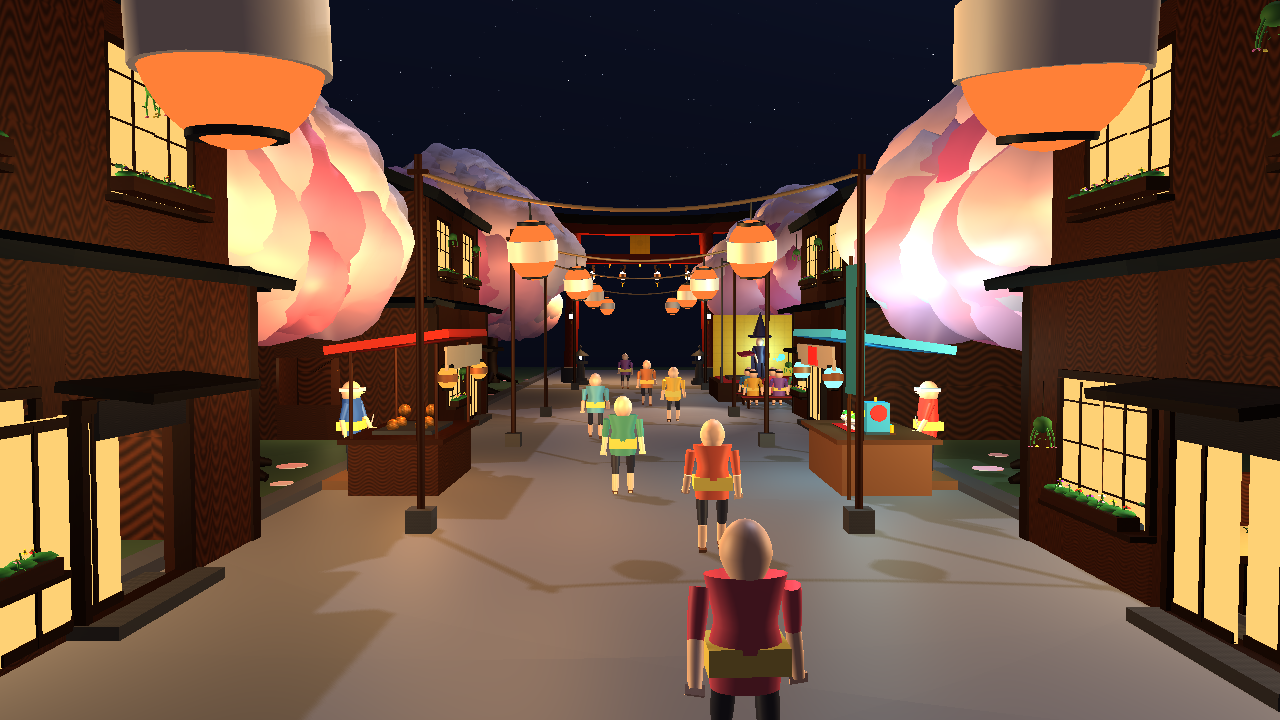
\includegraphics[width=\textwidth]{figures/ss_11_shading_blinn_phong.png}%
  }{\fbox{ss\_11}}
  \caption{Blinn-Phong (Mode 0)}
  \label{fig:shading_bp}
\end{subfigure}\hfill
\begin{subfigure}[b]{0.32\textwidth}
  \centering
  \IfFileExists{figures/ss_12_shading_diffuse_only.png}{%
    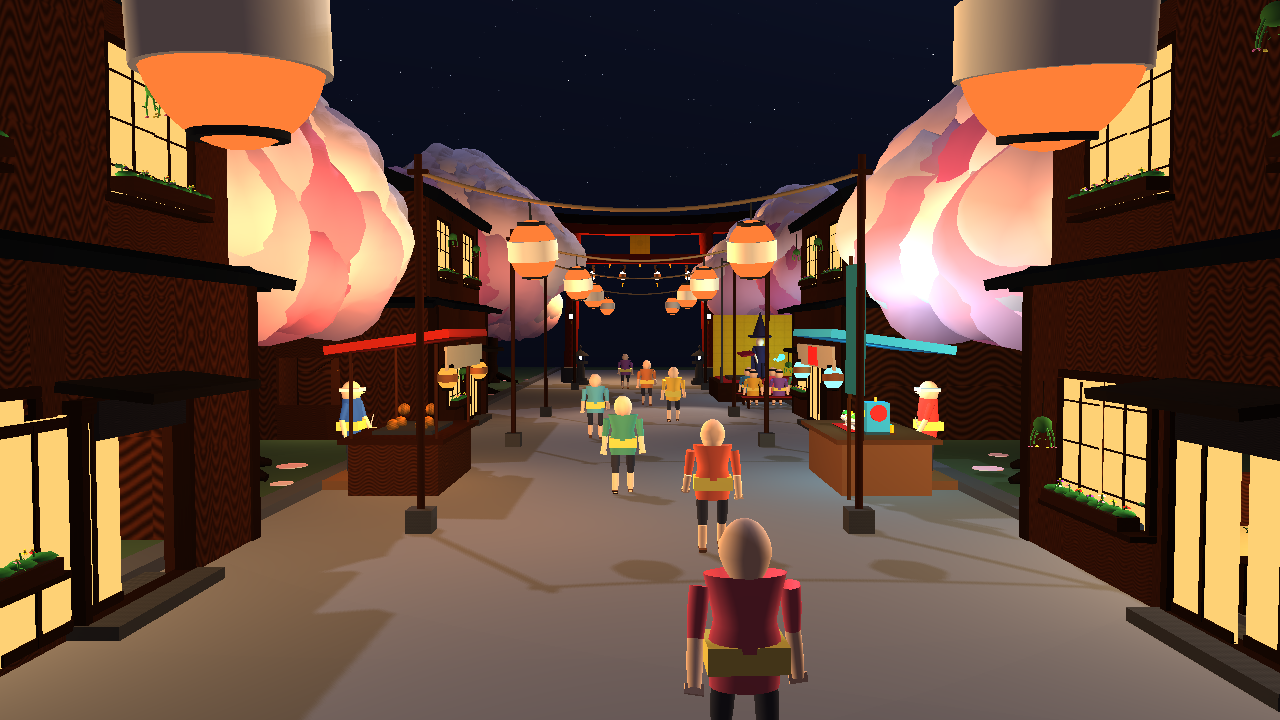
\includegraphics[width=\textwidth]{figures/ss_12_shading_diffuse_only.png}%
  }{\fbox{ss\_12}}
  \caption{Diffuse-Only (Mode 1)}
  \label{fig:shading_diff}
\end{subfigure}\hfill
\begin{subfigure}[b]{0.32\textwidth}
  \centering
  \IfFileExists{figures/ss_13_shading_ambient_only.png}{%
    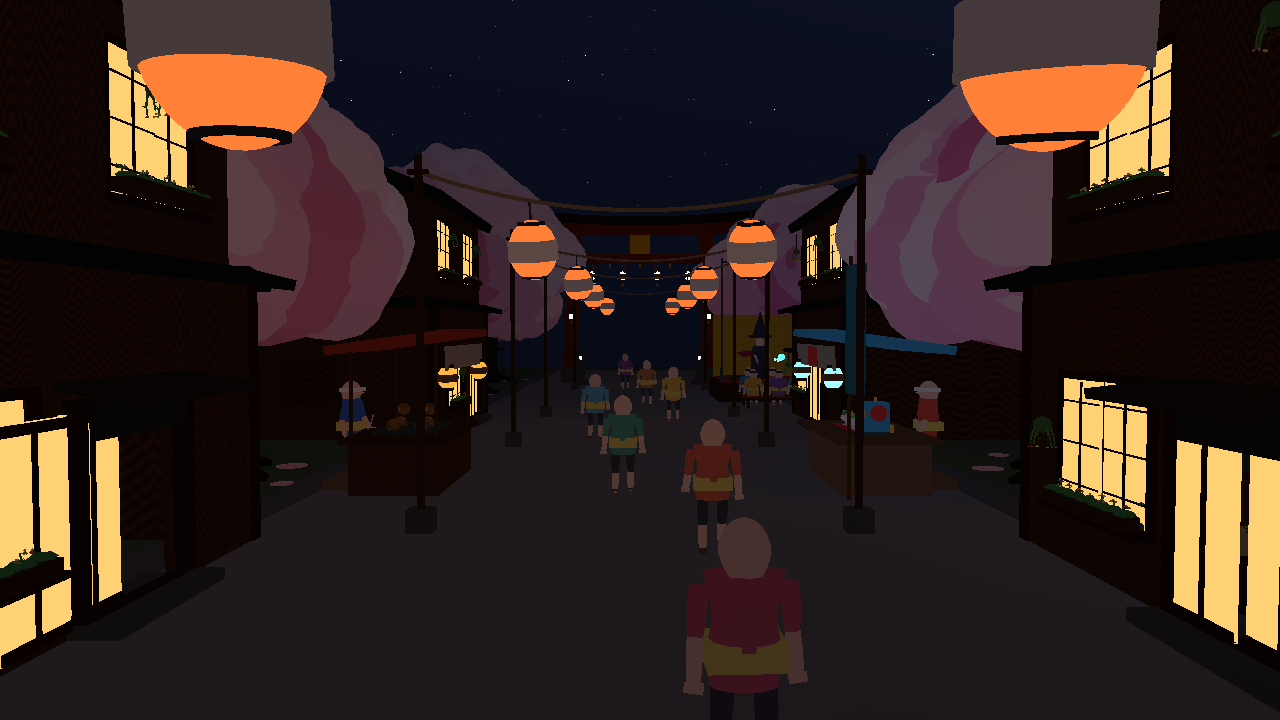
\includegraphics[width=\textwidth]{figures/ss_13_shading_ambient_only.png}%
  }{\fbox{ss\_13}}
  \caption{Ambient-Only (Mode 2)}
  \label{fig:shading_amb}
\end{subfigure}
\caption{Visual comparison of the three runtime shading modes accessible via Key P.}
\label{fig:shading_comparison}
\end{figure}

\section{Day / Night Sky Dome and Atmospheric Transition}
Pressing the \textbf{N} key smoothly drives the state variable \texttt{dayNightFactor} between $0.0$ (Daylight) and $1.0$ (Festival Night). Figure~\ref{fig:day_night_curves_diagram} plots the modulation of celestial and artificial light intensities across this transition.

\begin{figure}[htbp]
\centering
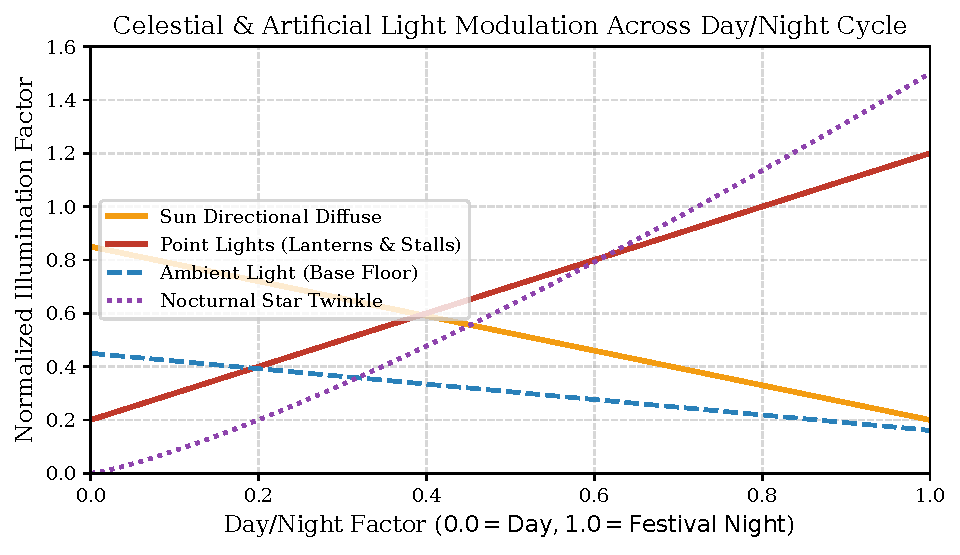
\includegraphics[width=0.52\textwidth]{figures/fig_day_night_curves.pdf}
\caption{Continuous light modulation curves across the Day/Night state transition.}
\label{fig:day_night_curves_diagram}
\end{figure}

\subsection{Procedural Celestial Bodies}
The celestial sphere (\texttt{isSky == true}) evaluates view direction $\mathbf{V} = \operatorname{normalize}(\mathbf{p}_{\text{frag}} - \mathbf{p}_{\text{cam}})$:
\begin{itemize}
    \item \textbf{Celestial Sun (Daylight):} Emits a sharp core disc when $\mathbf{V} \cdot \mathbf{D}_{\text{sun}} > 0.9972$ with a wide exponential atmospheric corona bloom $(\mathbf{V}\cdot\mathbf{D}_{\text{sun}})^{64} \times 1.10$.
    \item \textbf{Celestial Moon (Nighttime):} Silvery-white disc with a crater modulation function $\sin(16u)\cos(18v) \times 0.12$ and an ethereal bluish outer halo.
    \item \textbf{Twinkling Starfield:} Evaluated across two spatial grid frequencies ($160\times$ and $320\times$). A pseudo-random hash generator extracts star seeds, animating individual brightnesses with sinusoidal twinkle frequencies:
    \begin{equation}
    I_{\text{star}} = \operatorname{smoothstep}(r_{\text{star}}, 0, d) \cdot \left[ 0.65 + 0.35 \sin(\omega t + \phi) \right] \cdot \operatorname{pow}(\text{dayNightFactor}, 1.25)
    \end{equation}
\end{itemize}

\begin{figure}[htbp]
\centering
\begin{subfigure}[b]{0.48\textwidth}
  \centering
  \IfFileExists{figures/ss_01_overview_day.png}{%
    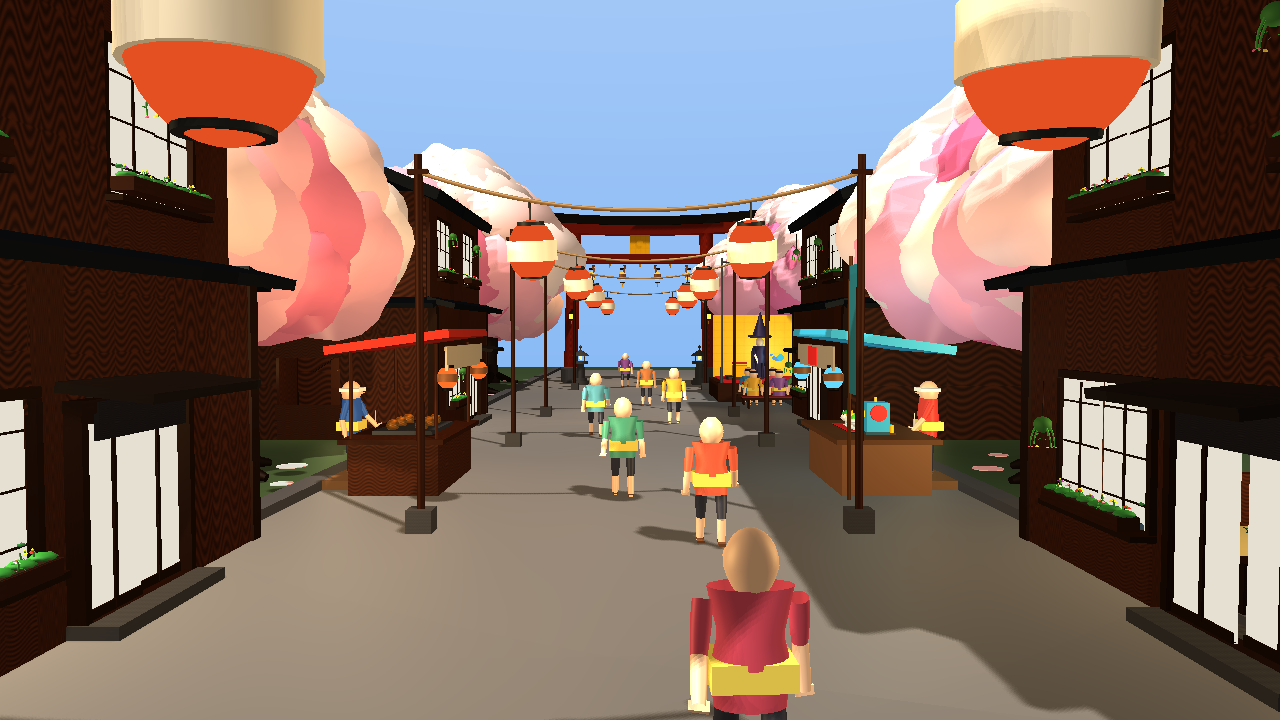
\includegraphics[width=\textwidth]{figures/ss_01_overview_day.png}%
  }{\fbox{ss\_01}}
  \caption{Daytime View (Factor = 0.0)}
  \label{fig:overview_day}
\end{subfigure}\hfill
\begin{subfigure}[b]{0.48\textwidth}
  \centering
  \IfFileExists{figures/ss_02_overview_night.png}{%
    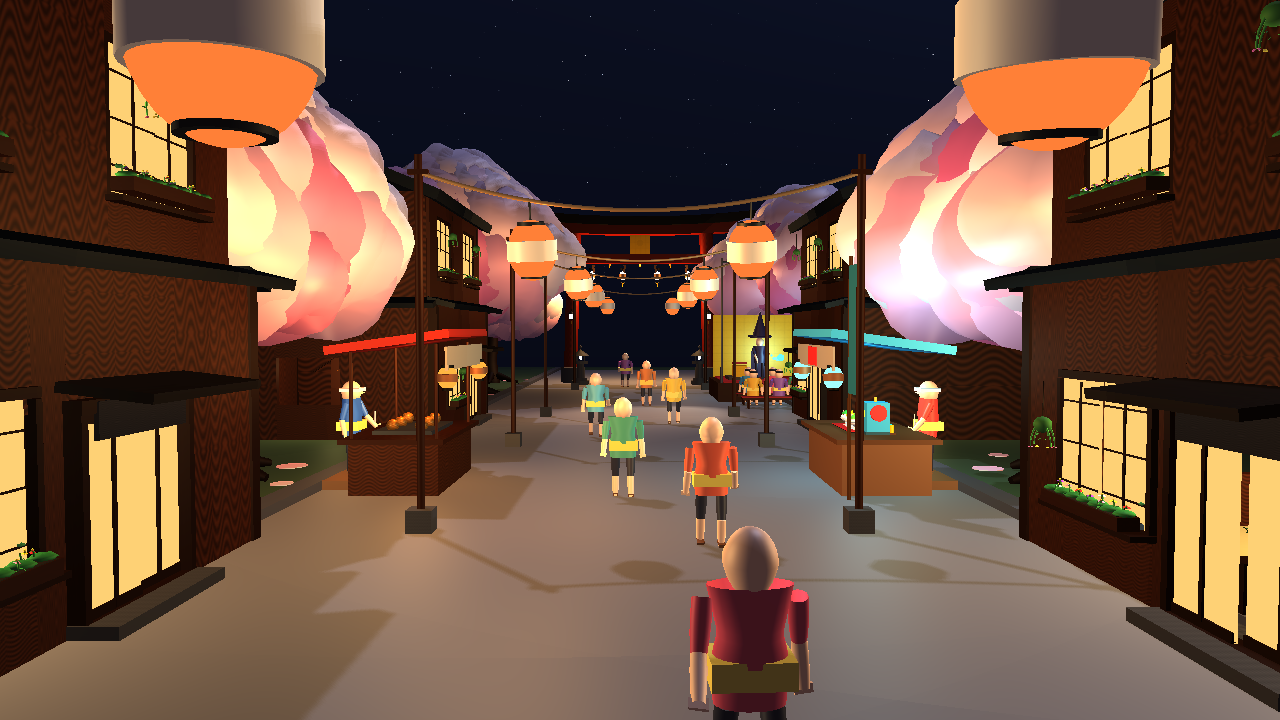
\includegraphics[width=\textwidth]{figures/ss_02_overview_night.png}%
  }{\fbox{ss\_02}}
  \caption{Festival Night View (Factor = 1.0)}
  \label{fig:overview_night}
\end{subfigure}
\caption{Comparison of the festival street under bright daytime and nocturnal illumination.}
\label{fig:day_night_comparison}
\end{figure}

\section{Specialized Material Shading Models}
\begin{enumerate}
    \item \textbf{Shoji Paper Translucency (\texttt{isWindow}):} Traditional sliding paper screens transmit interior and exterior light. In daytime, screens appear as crisp neutral parchment; at night, indoor lamps (Point Lights 6--11) back-illuminate screens into glowing warm amber radiators ($1.0, 0.82, 0.45$).
    \item \textbf{Emissive Materials (\texttt{isEmissive}):} Chochin paper lanterns and firework sparks emit radiant self-illumination independent of directional shadow occlusion.
    \item \textbf{Indoor Ambient Bounce:} To prevent interiors from becoming pitch-black cavities when doors or windows are open, the shader blends a warm ambient bounce color:
    \begin{equation}
    \mathbf{I}_{\text{indoorBounce}} = \operatorname{mix}\left( [0.48, 0.45, 0.40]^T, [0.18, 0.16, 0.14]^T, \text{dayNightFactor} \right) \cdot \mathbf{k}_d
    \end{equation}
\end{enumerate}
